\chapter{Mathematical model}
\label{sec:math}


\section{Transfer function for coil rig}

The schematic shown in \cref{fig:spolerigg11} is the schematic for the coil rig.

\begin{figure}[h!]
    \centering
    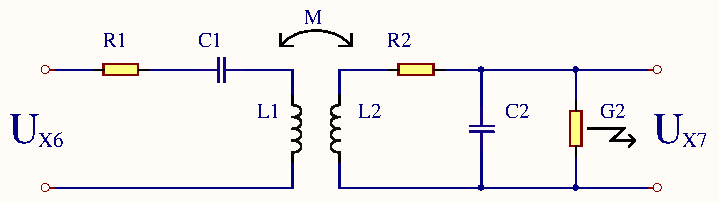
\includegraphics[width=\textwidth]{Skjema/Spolerigg1_r.pdf}
    \caption{Caption}
    \label{fig:spolerigg11}
\end{figure}

R1 is the resistance in the primary circuit (mainly the cable from the driver to the coil rig), R2 is the resistance in the secondary circuit (mainly the resistance in L2). C1 is the primary capacitor, L1 is the primary coil, L2 is the secondary coil, and C2 is the secondary capacitance (or top load). G1 is the electrical arc modelled as a conductance, see \cref{eq:g1} for the model of G1, this model is a combination of Cassie \citep{cassie} and Mayr \citep{mayr} models for electrical arcs presented in \citep{575670}. $U_{X6}$ is the voltage output from the driver to the primary resonant circuit, $U_{X7}$ is the voltage output from the secondary resonant circuit (the voltage driving the electrical arc).

This schematic can be simplified by introducing the mutual inductance M as a component as shown in \cref{fig:spolerigg2}, and then further simplified by representing the branches of the circuit as impedances as shown in \cref{fig:spolerigg3}.

\begin{figure}[h!]
    \centering
    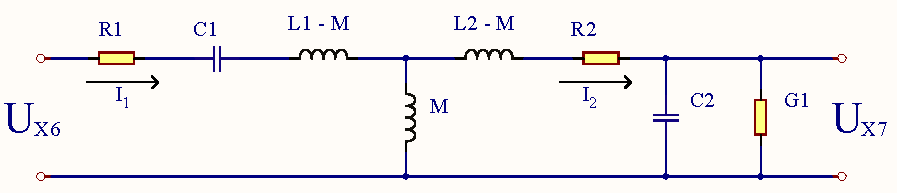
\includegraphics[width=\textwidth]{Skjema/Spolerigg2_r.pdf}
    \caption{Caption}
    \label{fig:spolerigg2}
\end{figure}

\begin{figure}[h!]
    \centering
    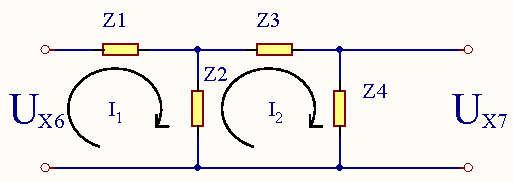
\includegraphics[width=\textwidth]{Skjema/Spolerigg3_r.pdf}
    \caption{Caption}
    \label{fig:spolerigg3}
\end{figure}

Using the mesh current method we get \cref{eq:1} and \cref{eq:2}.

\begin{equation} \label{eq:1}
    U_{X6} - I_1 Z_1 - (I_1 - I_2) Z_2 = 0
\end{equation}

\begin{equation} \label{eq:2}
    (I_2 - I_1) Z_2 - I_2 Z_3 - I_2 Z_4 = 0
\end{equation}

We then solve these two equations for $I_1$. Set \cref{eq:1_2} equal to \cref{eq:2_2}, solve for $\frac{U_{X7}}{U_{X6}}$ and substitute in \cref{eq:3}.

\begin{equation} \label{eq:3}
    U_{X7} = I_2 Z_4
\end{equation}

\begin{equation} \label{eq:1_2}
    I_1 = \frac{U_{X6} + I_2 Z_2}{Z_1 + Z_2}
\end{equation}'

\begin{equation} \label{eq:2_2}
    I_1 = \frac{(Z_2 - Z_3 - Z_4) I_2}{Z_2}
\end{equation}

We then have the transfer function $H(s)$ for the coil rig \cref{eq:4}.

\begin{equation} \label{eq:4}
    \frac{U_{X7}}{U_{X6}} = H(s) = \frac{Z_2 \cdot Z_4}{Z_1 \cdot (Z_2 - Z_3 - Z_4) - Z_2 \cdot (Z_3 + Z_4))}
\end{equation}

where

\begin{equation} \label{eq:4_1}
    Z_1 = R_1 + \frac{1}{s C_1} + s L_1 - s M,
\end{equation}

\begin{equation} \label{eq:4_2}
    Z_2 = s M,
\end{equation}

\begin{equation} \label{eq:4_3}
    Z_3 = s L_2 - s M + R_2,
\end{equation}

\begin{equation} \label{eq:4_4}
    Z_4 = \frac{1}{s C_2} + \frac{1}{G_1},
\end{equation}

\begin{equation} \label{eq:4_5}
    M = k \sqrt{L_1 L_2}.
\end{equation}

%\begin{equation}
%    H(s) = \frac{s M (\frac{1}{s C_2} + \frac{1}{G_1})}{(R_1 + \frac{1}{s C_1} + s L_1 - s M) \cdot (s M - (s L_2 - s M + R_2) - (\frac{1}{s C_2} + \frac{1}{G_1})) - s M \cdot ((s L_2 - s M + R_2) + (\frac{1}{s C_2} + \frac{1}{G_1})))}
%\end{equation}

% (Z2*Z4)/(Z1*(Z2-Z3-Z4)-Z2*(Z3+Z4)), Z1=(R1+1/(s*C1)+s*L1-s*M), Z2=(s*M, Z3=(s*L2)-(s*M)+R2), Z4=(1/(s*C2))+(1/G1))
However to be able to analyze this transfer function we have to order it into standard form. Meaning isolating $s$,$s^2$,$s^3$ etc. and expanding the factors. This leads to \cref{eq:5}.

%\begin{equation}
%    H(s) = \frac{s^2 M C_1}{s^4(2 M L_1 C_2 C_1 - L_1 L_2 C_2 C_1) + s^3(2 M R_1 C_2 C_1 - L_2 R_1 C_2 C_1 + 2 M L_1 G_1 C_1 - L_1 R_2 C_2 C_1) + s^2(2 M R_1 G_1 C_1 - R_1 R_2 C_2 C_1 + 2 M C_2 - C_2 L_2 - L_1 R_2 G_1 C_1 - L_1 C_1 + 2 M C_1) + s(2 M G_1 - R_1 R_2 G_1 C_1 - R_1 C_1 - L_2 G_1) - R_2 G_1- 1}
%\end{equation}

\begin{equation} \label{eq:5}
    H(s) = \frac{s^3 f + s^2 g}{s^4 a + s^3 b + s^2 c + s d + e}
\end{equation}

where

\begin{equation} \label{eq:5_1}
    a = (C_1 C_2 G_1 L_1 L_2)-2 (C_1 C_2 G_1 L_1 M)+(C_1 C_2 G_1 M^2),
\end{equation}

\begin{equation} \label{eq:5_2}
    b = (C_1 C_2 G_1 L_1 R_2)+(C_1 C_2 G_1 L_2 R_1)-2 (C_1 C_2 G_1 M R_1)+(C_1 C_2 L_1),
\end{equation}

\begin{equation} \label{eq:5_3}
    c = (C_1 C_2 G_1 R_1 R_2)+(C_1 C_2 R_1)+(C_1 G_1 L_1)+(C_2 G_1 L_2)-2 (C_2 G_1 M),
\end{equation}

\begin{equation} \label{eq:5_4}
    d = (C_1 G_1 R_1)+(C_2 G_1 R_2)+C_2,
\end{equation}

\begin{equation} \label{eq:5_5}
    e = G_1,
\end{equation}

\begin{equation} \label{eq:5_6}
    f = C_1 C_2 M,
\end{equation}
and
\begin{equation} \label{eq:5_7}
    g = C_1 G_1 M.
\end{equation}

Orders of magnitude for the parameters in the transfer function is shown in \cref{tab:mod_params} these sizes are rounded approximate sizes for a DRSSTC.

\begin{table}[]
    \centering
    \begin{tabular}{c|c|c|c}
         & Comment &  &\\ \hline
        C1 & Primary load capacitor                 & $10^{-7}$ & F \\
        C2 & Secondary load capacitor (top load)    & $10^{-11}$& F \\
        L1 & Primary coil                           & $10^{-5}$ & H \\
        L2 & Secondary coil                         & $10^{-1}$ & H \\
        M  & Mutual inductance                      & $10^{-6}$ & H \\
        R1 & Primary circuit ohmic resistance       & $10^{1}$  & $\Omega$ \\
        R2 & Secondary circuit ohmic resistance     & $10^{2}$  & $\Omega$ \\
        G1 & Conductance of elecrical arc           & $10^{-6}$  & $\Omega$ \\
        k  & Coupling factor                        & $10^{-1}$ & 
    \end{tabular}
    \caption{Model parameter sizes}
    \label{tab:mod_params}
\end{table}

\todo{Forklare hvorfor disse størrelsene}

Shown in \cref{fig:bode} is the bode plot of the transfer function $H(j\omega)$ \cref{eq:5} of the resonant circuit with the orders of magnitude in \cref{tab:mod_params}.

\begin{figure}[H]
    \centering
    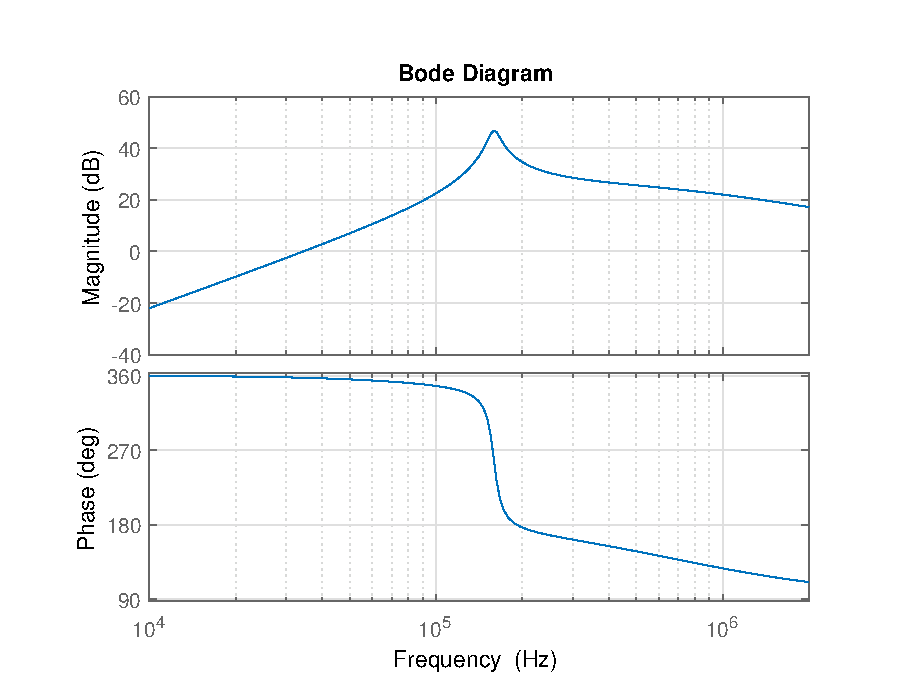
\includegraphics[width=\textwidth]{img/CoilRigBode.eps}
    \caption{Bode plot of $H(j\omega)$}
    \label{fig:bode}
\end{figure}

Here we see that the frequency response takes the form of a resonant circuit with a resonant frequency $f_0$ of 157kHz, which is close to the frequency one would expect with the orders of magnitude given in \cref{tab:mod_params} and the equation for resonance frequency \cref{eq:f0} of 160kHz. The magnitude at resonance is 36,7dB and then flattens at a magnitude 26dB at frequencies higher than resonance.

\begin{equation} \label{eq:f0}
    f_0 = \frac{1}{2 \pi \sqrt{L_1 C_1}}
\end{equation}

\todo{Skriv om å variere parametre}
\todo{Varier G1 fra 1e-5 til 1e-6}

In \cref{fig:step}, we see the step and impulse responses of the transfer function $H(j\omega)$ for the resonant circuit.

\begin{figure}[H]
    \centering
    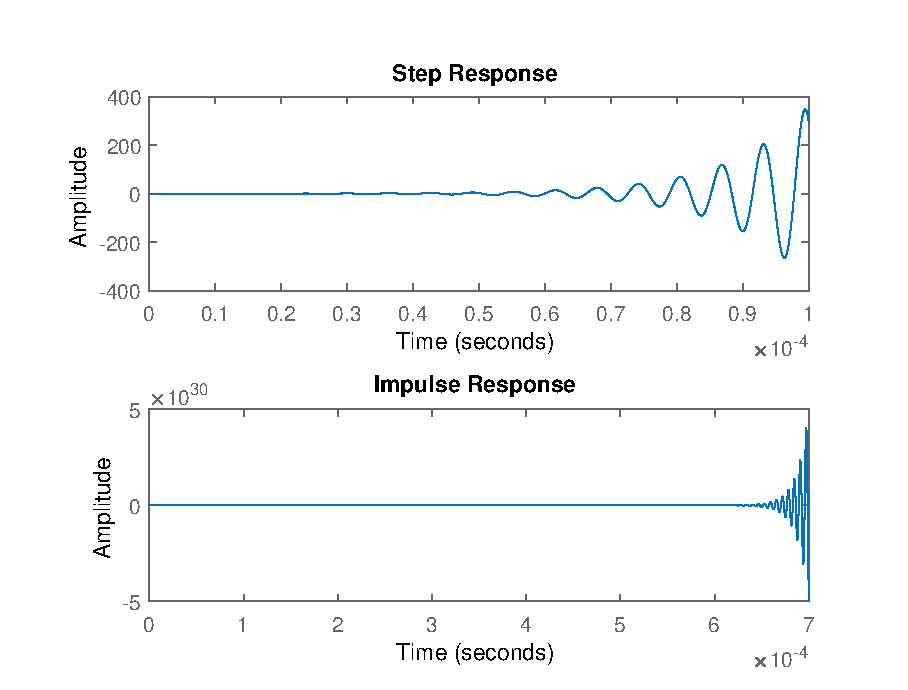
\includegraphics[width=\textwidth]{img/CoilRigResponse.eps}
    \caption{Step and impulse response for $H(j\omega)$}
    \label{fig:step}
\end{figure}

Here we see that we have a damped sinusiodal response with a frequency $f_s$ of 156kHz witch is the same frequency as the resonance frequency $f_0$ of the frequency response. This response attenuates within a few cycles.

\Cref{fig:polezero} shows the poles and zeros of the transfer function $H(j\omega)$ of the resonant circuit.

\begin{figure}[H]
    \centering
    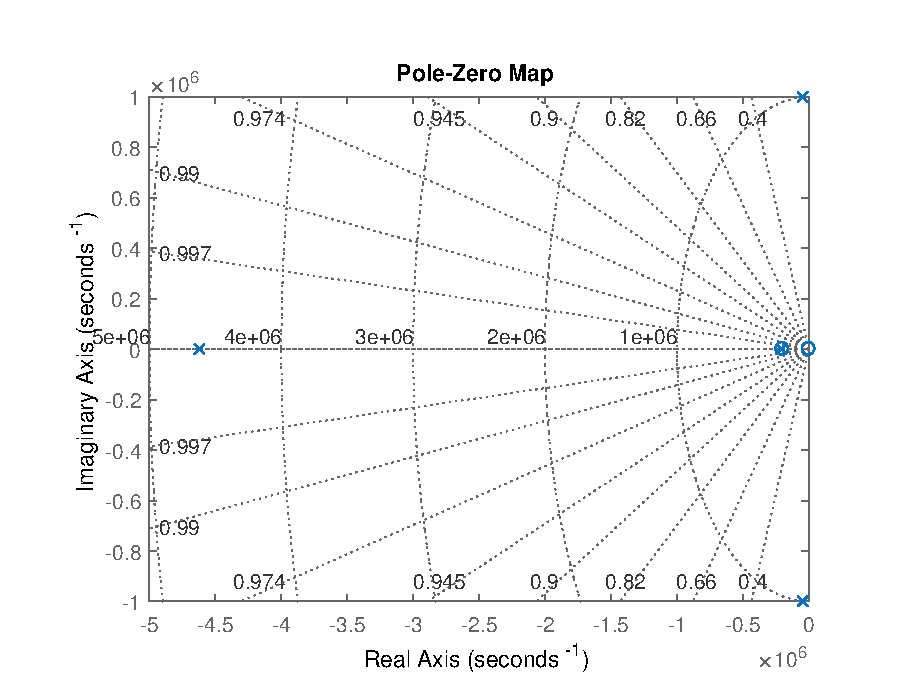
\includegraphics[width=\textwidth]{img/CoilRigPoleZeroPlot.eps}
    \caption{PoleZeroPlot for $H(j\omega)$}
    \label{fig:polezero}
\end{figure}

\Cref{tab:coilrigpoles} shows the numerical values of the poles and zeros of the transfer function $H(j\omega)$ of the resonant circuit.

\begin{table}[h]
    \centering
    \begin{tabular}{c|c}
        Poles & Zeros \\
        $(-1,4 + 9,6i)\cdot 10^{5} s^{-1}$ & $0$ \\
        $(-1,4 - 9,6i)\cdot 10^{5} s^{-1}$ & $0$ \\
        $(-2,1 + 0i)\cdot 10^{5} s^{-1}$ & $-2\cdot 10^{5} s^{-1}$ \\
    \end{tabular}
    \caption{Poles and zeros for $H(j\omega)$}
    \label{tab:coilrigpoles}
\end{table}

Here we observe a pole pair in the left half plane, a single real pole in the left half plane. As well as three zeros, one in the left half plane and two in origo.

\Cref{fig:crlinsim} shows the result of a linear simulation of the transfer function of the resonant circuit with a 160V peak square wave input signal with amplitude 1 and frequency 159kHz.

\begin{figure}[H]
    \centering
    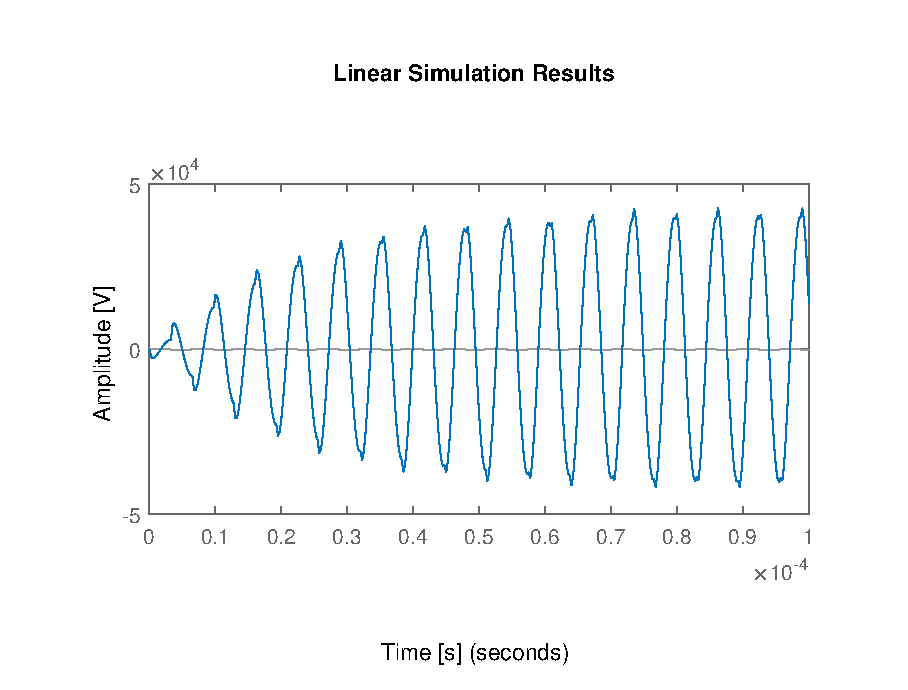
\includegraphics[width=\textwidth]{img/CoilRigSimulation.eps}
    \caption{Linear simulation of transfer function with square wave with $f=f_0$ as input}
    \label{fig:crlinsim}
\end{figure}

We see here that the output signal X6 starts with a quarter period of the step response shown in \cref{fig:step}, and then when the voltage peaks, meaning when the differential of the voltage is zero, a new step response with opposite phase is added to the output signal. This makes the output signal grow rapidly for three cycles to 160kV, before flattening out at 170kV.

\newpage
\section{Transfer function for feedback}
\label{sec:mod_fb}
If we use \cref{eq:1} and \cref{eq:2} and solve for $\frac{I_1}{U_{X6}}$ we get the transfer function for the feedback signal shown in \cref{eq:fb_1} to \cref{eq:fb_q}. Where $Z_1$ to $Z_4$ are the same impedances as given in \cref{eq:4}.

\begin{equation} \label{eq:fb_1}
\frac{I_1}{U_{X6}} = H_{FB}(s) = \frac{Z_2-Z_3-Z_4}{(Z_1+Z_2)(Z_2-Z_3-Z_4)-Z_2^2}
\end{equation}

\begin{equation} \label{eq:fb_2}
    H_{FB}(s) = \frac{s^3 h + s^2 k + s l}{s^4 m + s^3 n + s^2 o + s p + q}
\end{equation}

Where

\begin{equation}
    h = 2(C_1 C_2 G_1 M) - (C_1 C_2 G_1 L_2)
\end{equation}

\begin{equation}
    k = -(C_1 C_2 G_1 R_2) - (C_1 C_2)
\end{equation}

\begin{equation}
    l = -C_1 G_1
\end{equation}

\begin{equation}
    m = (C_1 C_2 G_1 L_1 L_2)-2(C_1 C_2 G_1 L_1 M)
\end{equation}

\begin{equation} \label{eq:fb_n}
    n = (C_1 C_2 G_1 L_1 R_2) + (C_1 C_2 L_1) + (C_1 C_2 G_1 R_1 L_2) - 2(C_1 C_2 G_1 R_1 M)
\end{equation}

\begin{equation} \label{eq:fb_o}
    o = (C_1 G_1 L_1) + (C_1 C_2 R_1) + (C_2 G_1 L_2) -2(C_2 G_1 M)
\end{equation}

\begin{equation} \label{eq:fb_p}
    p = (C_1 G_1 R_1) + (C_2 G_1 R_2) + C_2
\end{equation}

\begin{equation} \label{eq:fb_q}
    q = G_1
\end{equation}

\Cref{fig:fb_bode} Shows the bode plot for the transfer function $H_{FB}(j\omega)$ for the feedback signals X8 and X9 (both are identical).

\begin{figure}[H]
    \centering
    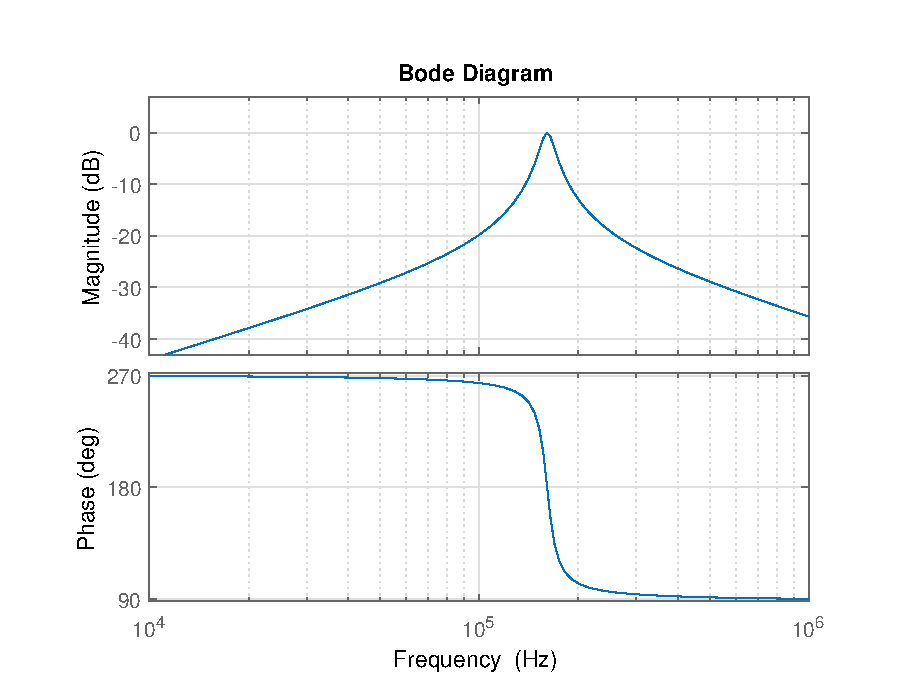
\includegraphics[width=\textwidth]{img/FeedBackBode.eps}
    \caption{Bode plot of the transfer function for the feedback signals $H_{FB}(j\omega)$}
    \label{fig:fb_bode}
\end{figure}

Here we see a much sharper peak at the resonant frequency than in the bode plot for the resonant circuit $H(j\omega)$. We also see that the response does not flatten at frequencies higher than the resonance frequency. The resonant frequency $f_0$ is 160kHz and the magnitude is 0dB at resonance.


\Cref{fig:fb_step} shows the step and impulse response of the feedback transfer function $H_{FB}(j\omega)$.

\begin{figure}[H]
    \centering
    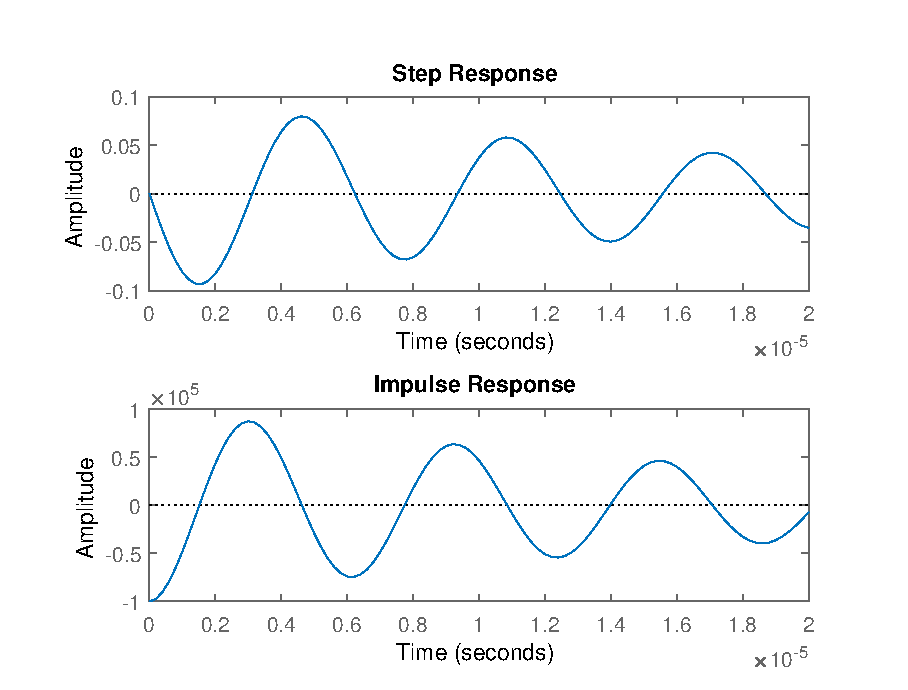
\includegraphics[width=\textwidth]{img/FeedBackResponse.eps}
    \caption{Step and impulse response of transfer function for the feedback current}
    \label{fig:fb_step}
\end{figure}

Here we see a damped sinusoiodal response with a frequency $f_s$ of 167kHz witch is slightly higher than the resonant frequency $f_0$ of 160kHz. The step response of the feedback signal attenuates slower than the step response of the resonant circuit.

\Cref{fig:fbpolezero} shows the pole and zero plot for the transfer function for the feedback signals $H_{FB}(j\omega)$.

\begin{figure}[H]
    \centering
    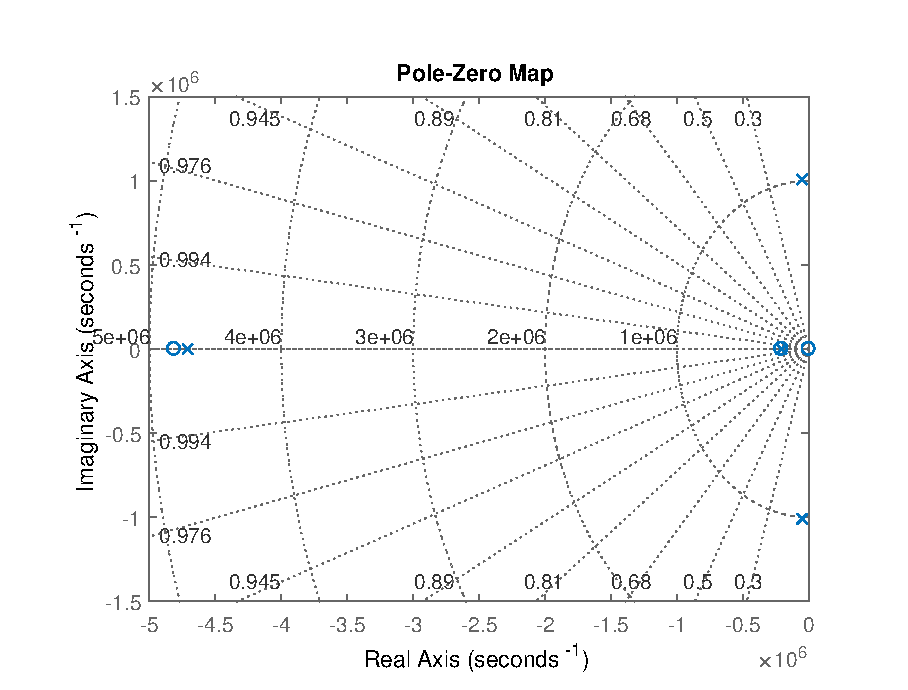
\includegraphics[width=\textwidth]{img/FeedBackPoleZeroPlot.eps}
    \caption{PoleZeroPlot for $H_{FB}(j\omega)$}
    \label{fig:fbpolezero}
\end{figure}

\Cref{tab:fbcoilrigpoles} shows the numerical values of the poles and zeros of the transfer function for the feedback signals $H_{FB}(j\omega)$.

\begin{table}[h]
    \centering
    \begin{tabular}{c|c}
        Poles & Zeros \\
        $(-47 + 0i)\cdot 10^{5} s^{-1}$ & \\
        $(-0,5 + 10i)\cdot 10^{5} s^{-1}$ & $0$ \\
        $(-0,5 - 10i)\cdot 10^{5} s^{-1}$ & $-48\cdot 10^{5} s^{-1}$ \\
        $(-2,1 + 0i)\cdot 10^{5} s^{-1}$ & $-2,1\cdot 10^{5} s^{-1}$ \\
    \end{tabular}
    \caption{Poles and zeros for $H_{FB}(j\omega)$}
    \label{tab:fbcoilrigpoles}
\end{table}

Here we observe a pole pair in the left half plane, two real poles in the left half plane. As well as three zeros, two in the left half plane and one in origo.

\Cref{fig:fblinsim} shows the result of a linear simulation of the transfer function of the feedback signal with a 160V peak square wave input signal with amplitude 1 and frequency 159kHz.

\begin{figure}[H]
    \centering
    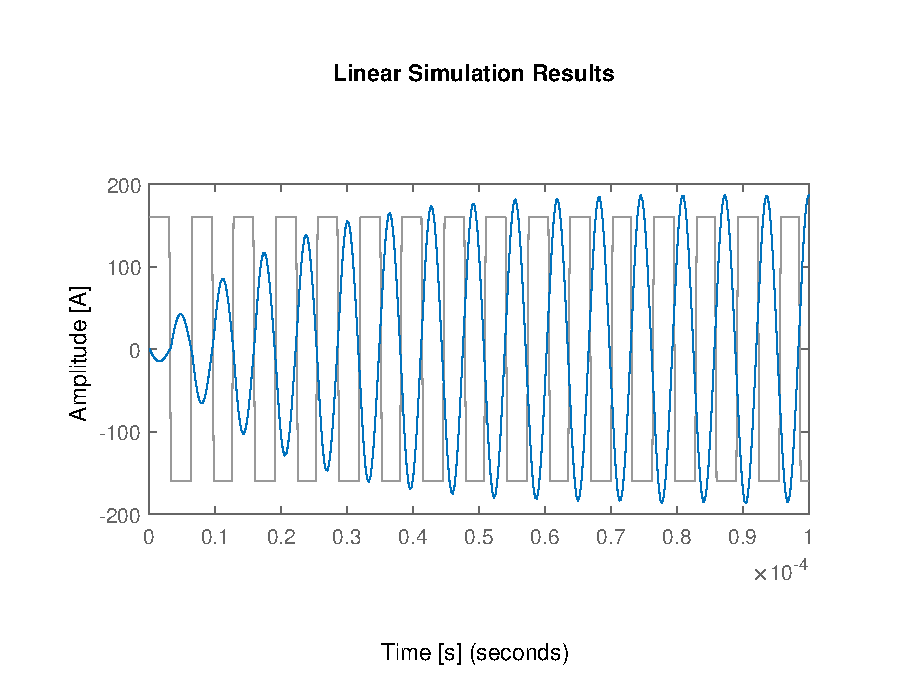
\includegraphics[width=\textwidth]{img/FeedBackSimulation.eps}
    \caption{Linear simulation of transfer function with square wave with $f=f_0$ as input}
    \label{fig:fblinsim}
\end{figure}

Here we see a sinusoidal current that grows rapidly for 9 cycles to 182A then stabilizes at 186A. We also see that the input signal switches when the current is zero, though after some cycles the input signal drifts out of sync with the current.

\newpage
\section{Magnitude analysis}
By taking the magnitudes for each variable listed in \cref{tab:mod_params} and inserting them into the different terms in the transfer function $H(s)$ (\cref{eq:4}) we can see witch terms influence the result and witch terms are insignificant. In \cref{tab:termsh} the values of each of the terms making up the main terms in \cref{eq:4}, are listed after inserting the magninudes in \cref{tab:mod_params}. e, f, and g are not listed since they only have a single term each.

\begin{table}[H]
    \centering
    \begin{tabular}{c|c|c}
        a & $(C_1 C_2 G_1 L_1 L_2)$   & $2 \cdot 10^{-29}$ \\
          & $2 (C_1 C_2 G_1 L_1 M)$   & $8 \cdot 10^{-32}$ \\
          & $(C_1 C_2 G_1 M^2)$       & $8 \cdot 10^{-31}$ \\
        \hline
        b & $(C_1 C_2 G_1 L_1 R_2)$   & $2 \cdot 10^{-26}$ \\
          & $(C_1 C_2 G_1 L_2 R_1)$   & $2 \cdot 10^{-23}$ \\
          & $2 (C_1 C_2 G_1 M R_1)$   & $8 \cdot 10^{-26}$ \\
          & $(C_1 C_2 L_1)$           & $1 \cdot 10^{-23}$ \\
        \hline
        c & $(C_1 C_2 G_1 R_1 R_2)$   & $2 \cdot 10^{-20}$ \\
          & $(C_1 C_2 R_1)$           & $1 \cdot 10^{-17}$ \\
          & $(C_1 G_1 L_1)$           & $2 \cdot 10^{-17}$ \\
          & $(C_2 G_1 L_2)$           & $2 \cdot 10^{-17}$ \\
          & $2 (C_2 G_1 M)$           & $8 \cdot 10^{-20}$ \\
        \hline
        d & $(C_1 G_1 R_1)$           & $2 \cdot 10^{-11}$ \\
          & $(C_2 G_1 R_2)$           & $2 \cdot 10^{-14}$ \\
          & $C_2$                     & $1 \cdot 10^{-11}$ \\
    \end{tabular}
    \caption{Magnitudes of parameters in H(s)}
    \label{tab:termsh}
\end{table}

From \cref{tab:termsh} we see that the first term of $a$ is the largest, and the second and third terms are two and one orders smaller. Thus they are not significant and can be removed without reducing accuracy significantly. Further the first and third terms of $b$ are three orders smaller than the second and fourth terms and can be removed with the same reasoning. The second and fourth terms of $b$ are of the same magnitude and is thus equally significant. Two terms can be removed from $c$ and one term from $d$. e, f, and g only contains one term each and can not be simplified. This gives the simplified main parameters shown in \cref{eq:ab_simp} and \cref{eq:cd_simp}.

\begin{equation} \label{eq:ab_simp}
    a' = (C_1 C_2 G_1 L_1 L_2), b' = [(C_1 C_2 G_1 L_2 R_1)+(C_1 C_2 L_1)],
\end{equation}
\begin{equation} \label{eq:cd_simp}
    c' = [(C_1 C_2 R_1)+(C_1 G_1 L_1)+(C_2 G_1 L_2)], d' = [(C_1 G_1 R_1) + C_2]
\end{equation}

Inserting the magnitudes from \cref{tab:mod_params} in $H(s)$ both before and after simplifying gives the same result when rounded to one significant digit as shown in \cref{tab:beforeafter}.

\begin{table}[h!]
    \centering
    \begin{tabular}{c|c|c}
          & Before             & After \\ \hline
        a & $2 \cdot 10^{-29}$ & $2 \cdot 10^{-29}$ \\
        b & $3 \cdot 10^{-23}$ & $3 \cdot 10^{-23}$ \\
        c & $5 \cdot 10^{-17}$ & $5 \cdot 10^{-17}$ \\
        d & $3 \cdot 10^{-11}$ & $3 \cdot 10^{-11}$ \\
        e & $2 \cdot 10^{-05}$ & $2 \cdot 10^{-05}$ \\
        f & $2 \cdot 10^{-22}$ & $2 \cdot 10^{-22}$ \\
        g & $4 \cdot 10^{-16}$ & $4 \cdot 10^{-16}$ \\
    \end{tabular}
    \caption{Terms in H(s) before and after magnitude analysis with one significant digit}
    \label{tab:beforeafter}
\end{table}

\todo{a,b,c,d,e,f,og g er alle signifikante. Hvordan bevise?}

\section{Streamer}
\label{sec:arc}

When the electric discharge from the top load of the resonant circuit forms long threads or filaments in the air this is called a streamer discharge \citep{streamer}. When a streamer discharge happens this affects the resonant circuit, this influence is proposed modeled as a varying conductance. A model for this conductance is found from an article \citep{575670} combining two classical models for electric discharge. This model is shown in \cref{eq:g1},

\begin{equation} \label{eq:g1}
    G_1 = G_{min} + [ 1 - \exp(-\frac{i_{G1}^2}{I_0^2})] \frac{U_{X7} i_{G1}}{E_0^2} + [\exp(-\frac{i_{G1}^2}{I_0^2})] \frac{i_{G1}^2}{P_0} - \theta \frac{d G_1}{dt}
\end{equation}

where

\begin{equation}
    \theta = \theta_0 + \theta_1 exp(-\alpha |i|)
\end{equation}

and the parameters in this model are shown in \cref{tab:g1params}.

\begin{table}[h]
    \centering
    \begin{tabular}{c|c|c|c}
         & Comment &  &\\ \hline
        $G_{min}$ & Least possible conductance &  &\\
        $\theta$  & Streamer dampening factor &  &\\
        $I_o$     & Limit between large and small current &  &\\
        $E_0$     & Constant, steady state streamer voltage &  &\\
        $P_0$     & Constant power loss from streamer &  & \\
        $i_{G1}$  & Current flowing in streamer      &  & \\
        $U_{X7}$     & Voltage over streamer            &  &
    \end{tabular}
    \caption{Parameters for model for $G_1$}
    \label{tab:g1params}
\end{table}

$G_{min}$ is the least possible conductance from the top load $C_2$ to ground. This conductance is present before any streamers form as well as after streamers have formed.

\todo{Corona?}

\subsection{Streamer capacitance}
It is also proposed, based on the general consensus in the hobby community \citep{streamercapacitance}, that the streamer increases the capacitance of the top load $C_2$.

\begin{equation}
    C_2' = C_2 + C_s = C_2 + l C_u
\end{equation}

Where $C_s$ is the capacitance introduced by the streamer. $l$ is the length of the streamer in meters, $C_u$ is the capacitance of the streamer per meter. This is an approximation, the actual capacitance of the streamer can be calculated from the definition of capacitance and becomes a complicated equation that also dependts on the ration between length and width of the streamer \citep{thinstraight}. Two values for the capacitance per meter used in the hobby community are 25pF \citep{conner}, and 5pF \citep{scantesla}.

\section{Varying parameters}

\begin{figure}[H]
    \centering
    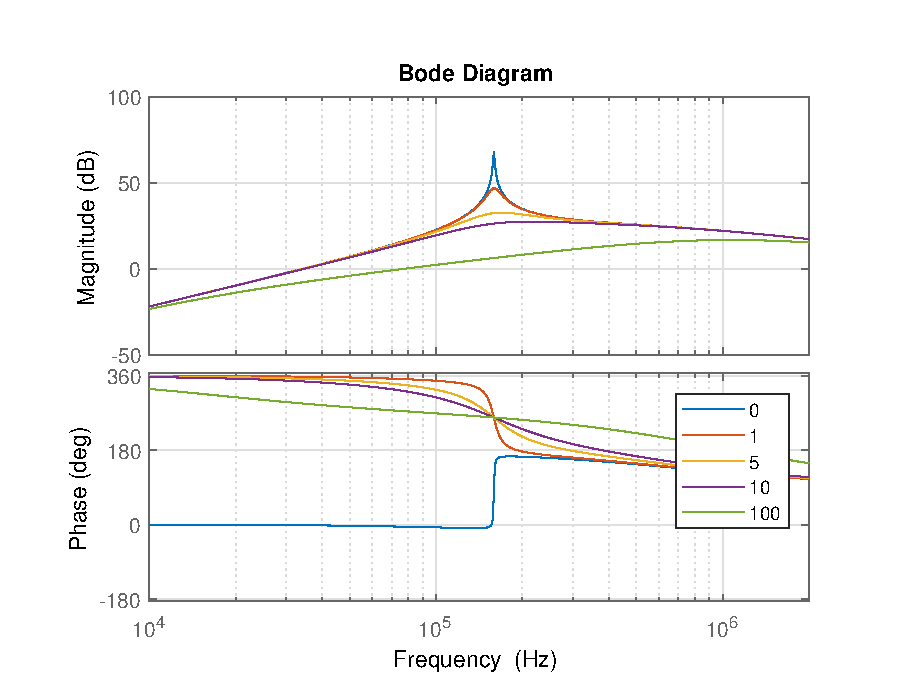
\includegraphics[width=\textwidth]{img/CoilRigBode_R1.eps}
    \caption{Bode plot of $H(j\omega)$ varying R1}
    \label{fig:bode_r1}
\end{figure}

\begin{figure}[H]
    \centering
    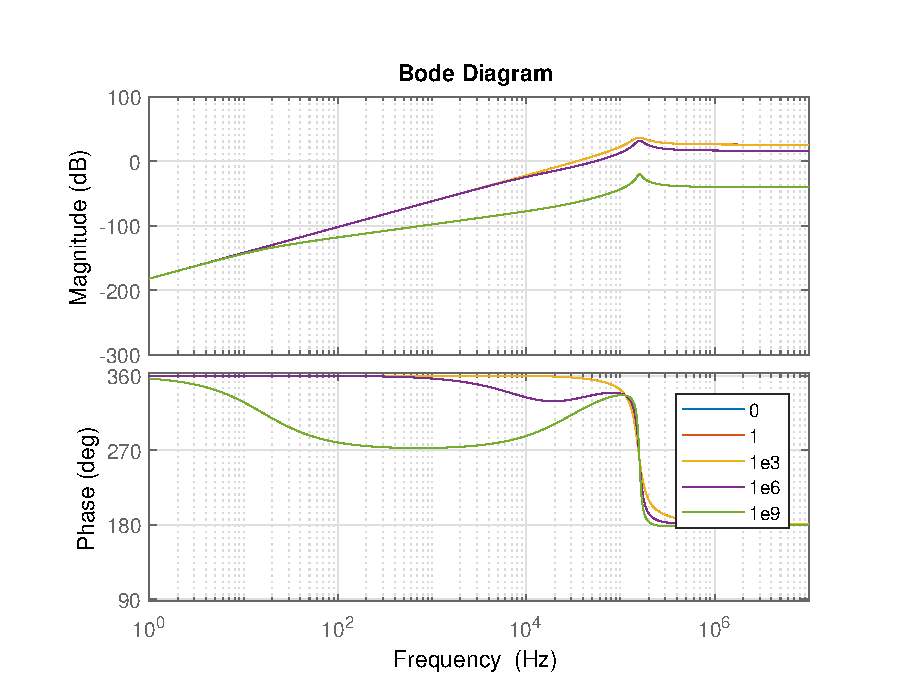
\includegraphics[width=\textwidth]{img/CoilRigBode_R2.eps}
    \caption{Bode plot of $H(j\omega)$ varying R2}
    \label{fig:bode_r2}
\end{figure}

\begin{figure}[H]
    \centering
    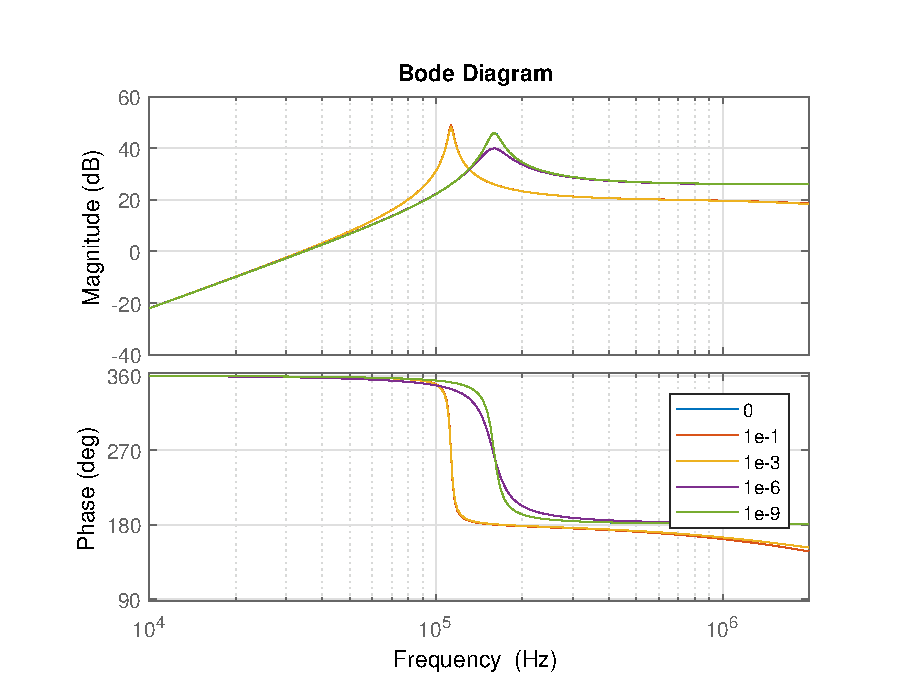
\includegraphics[width=\textwidth]{img/CoilRigBode_G1.eps}
    \caption{Bode plot of $H(j\omega)$ varying G1}
    \label{fig:bode_g1}
\end{figure}

\begin{figure}[H]
    \centering
    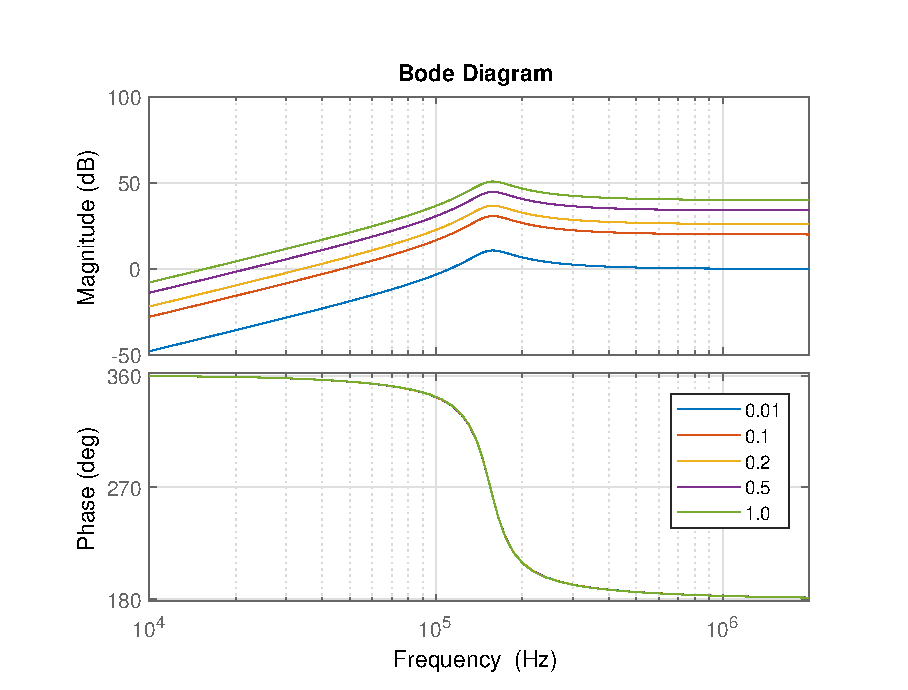
\includegraphics[width=\textwidth]{img/CoilRigBode_k.eps}
    \caption{Bode plot of $H(j\omega)$ varying k}
    \label{fig:bode_k}
\end{figure}
